\chapter{Estado del arte}
Para poder organizar este proyecto debemos conocer el estado del arte en su ámbito. Hablaremos del estado de arte en cheminformatics, las herramientas que se han creado en el marco de esta ciencia y las técnicas de Deep Learning que utilizamos para desarrollar el TFG.

\section{Cheminformatics}
Como comentamos en la introducción, cheminformatics es un tema muy amplio y engloba subtópicos diferentes. Muchos de ellos surgieron en la década de 1960 y principios de 1970, y desde esa época muchos grupos de investigación siguen trabajando en ellos y nuevos grupos han surgido para aplicar nuevas tecnologías en nuevos ámbitos. A continuación discutimos algunos de los temas que históricamente han sido de interés para esta ciencia. \cite{doi:10.1021/ci600234z}

\subsection{Compuestos orgánicos y su representación}
Un compuesto orgánico es un compuesto químico que contiene átomos de carbono, formando enlaces carbono-carbono y carbono-hidrógeno \cite{comporganico}. En este TFG, vamos a trabajar concretamente con la clasificación de compuestos organometálicos, donde los átomos de carbono forman enlaces covalentes con átomos metálicos \cite{comporganometalico}.

En las publicaciones de química encontramos numerosas representaciones gráficas de estos compuestos, lo que se conocen como fórmulas estructurales. Éstas muestran la disposición en el espacio de los átomos que forman el compuesto. Un ejemplo es la siguiente figura:

\begin{figure}[H]
\centering
    \fbox{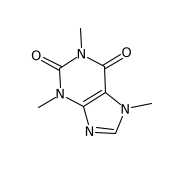
\includegraphics[scale=0.7]{imagenes/caffeine.png}}  
    \caption{Estructura de la cafeína}
\end{figure}

\noindent En ellas pueden aparecer multitud de elementos, apareciendo siempre:
\begin{itemize}
    \item \textbf{Átomos:} Se sitúan en los extremos de los enlaces. Representados con letras que indican el elemento químico del que se trata, tal y como aparece en la tabla periódica.
    \item \textbf{Enlaces:} Unen dos átomos entre sí. 
\end{itemize}

 En algunas ocasiones, sobre los átomos pueden mostrarse cargas positivas o negativas representando iones. Aparte, puede mostrarse lo que se conoce como información estereoquímica, que indica la disposición de los átomos en el espacio. Ésta es importante ya que afecta a las propiedades y reactividad de las moléculas \cite{estereoquimica,structrep}.

 \begin{figure}[H]
\centering
    \fbox{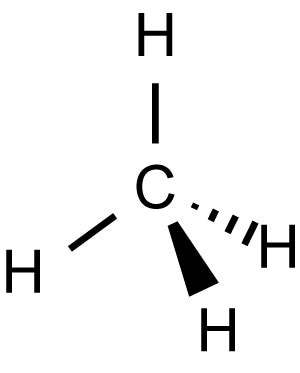
\includegraphics[scale=0.5]{imagenes/methane.jpg}}  
    \caption{Estructura del metano} 
\end{figure}

\begin{itemize}
    \item Las líneas sólidas representan enlaces en el plano.
    \item Las discontinuas representan enlaces que están más alejados.
    \item Aquellas con forma de cuña indican que uno de los átomos se encuentra más cerca del espectador. 
\end{itemize}

Además, un mismo compuesto se puede representar de distintas formas:
\begin{figure}[H]
\centering
    \fbox{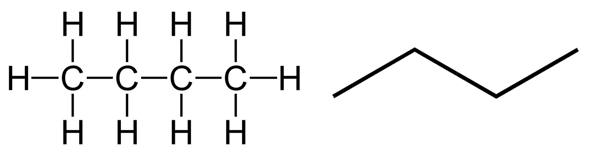
\includegraphics[scale=0.3]{imagenes/skeletal.png}}  
    \caption{Dos formas de representar el butano} 
\end{figure}

En a) se detalla la definición de todos los átomos, en cambio en b) encontramos lo que se conoce como fórmula de esqueleto, donde se omiten los átomos de carbono e hidrógeno. Se sabe que hay un átomo de carbono en los vértices que quedan libres en la intersección de dos enlaces o en las terminaciones donde no aparece ningún otro elemento. Se supone a la vez que cada átomo de carbono tiene cuatro enlaces, por tanto el número de enlaces que faltan por indicar explícitamente se corresponden con enlaces a moléculas de hidrógeno \cite{formestructural,structrep}.


\subsection{Representación en el ordenador}
El poder almacenar representaciones de compuestos químicos de manera eficiente en un ordenador requiere de la creación de métodos y formatos específicos para ello. Además, hay que tener en cuenta qué datos vamos a codificar, si solo la estructura básica del compuesto, si también queremos guardar información estereoquímica o si queremos añadir notas auxiliares sobre los compuestos. Es importante tener esto claro, ya que la complejidad de la representación influirá en la cantidad de almacenamiento que ocupe en disco y en los recursos necesarios para procesarla.

Utilizando notación lineal, representamos la estructura del compuesto como una secuencia lineal de caracteres y números. Esta es una codificación adecuada para las computadoras, ya que la pueden procesar con facilidad. Algunos formatos que utilizan esta notación son WLN (Wiswesser Line Notation), ROSDAL (Rp) o SMILES (Simplified Molecular Input Line Entry Specification). Aunque WLN y ROSDAL han quedado obsoletos, SMILES se sigue utilizando con mucha frecuencia en la actualidad. \cite{doi:10.1021/ci600234z}

\begin{figure}[H]
\centering
    \fbox{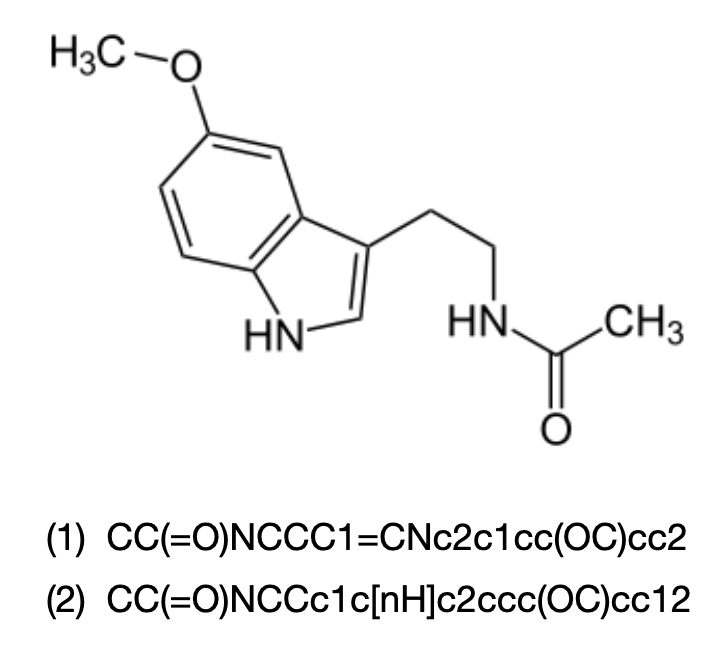
\includegraphics[scale=0.25]{imagenes/smiles_melatonina.png}}  
    \caption{Dos posibles codificaciones de la melatonina en SMILES \cite{smiles_wikipedia}}
\end{figure}

Aunque no vamos a entrar en detalle de cómo funciona, ya que para ello hay que tener nociones avanzadas de química, diremos que utiliza las siglas de cada elemento de la tabla periódica para representar los átomos. La primera letra del elemento se escribe en mayúscula, a no ser que se trate de un átomo perteneciente a un anillo aromático\footnote{La aromaticidad es una propiedad presente en enlaces dobles de moléculas cíclicas, donde sus electrones pueden circular libremente. Esto mejora la estabilidad del compuesto. \cite{aromaticidad, aromaticidad_wikipedia}}, ya que en ese caso se escribe en minúscula. Si el elemento tiene dos caracteres, el segundo se escribe siempre en minúscula. Además, se pueden representar cargas.

Los enlaces se representan con -, =, \# y :, según el tipo. Bajo algunas circunstancias, se pueden omitir estos símbolos, ya que por su contexto se deducen. También se pueden codificar ramas, situando elementos entre paréntesis, y ciclos, utilizando un número para indicar el inicio y el fin del ciclo en la cadena de texto. \cite{weininger1988smiles}

\begin{figure}[H]
\centering
    \fbox{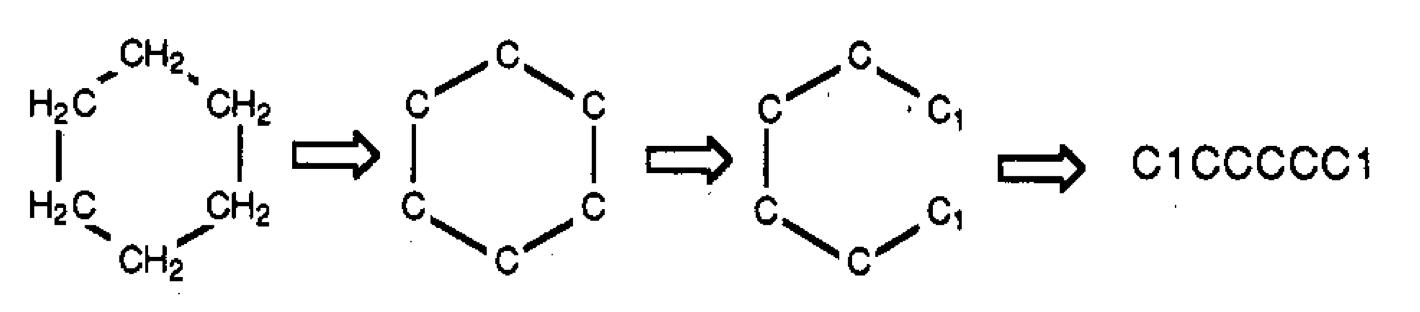
\includegraphics[scale=0.35]{imagenes/smiles_cycle.png}}  
    \caption{Ciclos en SMILES} 
\end{figure}

Otras características como la aromaticidad o estructuras inconectas también pueden ser representadas. Entre las ventajas de esta codificación, destaca su facilidad de comprensión por los humanos. Cualquier químico puede aprender sus reglas de codificación fácilmente y diseñar sus propios compuestos. Un problema que tiene SMILES es que un mismo elemento se puede representar de diferentes formas. Pero sobre todo, el mayor problema es que un porcentaje significativo de las cadenas no se corresponden con moléculas válidas, ya sea porque son sintácticamente inválidas, no se corresponden con un grafo molecular o no cumplen reglas químicas básicas. \cite{weininger1988smiles}

Uno de los principales objetivos de la química computacional es el diseño de nuevas moléculas. Para ello, la utilización de modelos generativos puede ayudar a los investigadores, pero si el espacio de estados de SMILES no es completamente válido se dificulta la tarea. Para ello han surgido otras codificaciones como SELFIES con un espacio 100\% robusto. \cite{Krenn_2020}

Además de estos formatos de notación lineal, es necesario mencionar otros. El lanzamiento en 1982 de MDL MOLfile llevó a su aceptación como principal formato para codificar compuestos químicos. Se han realizado distintas adaptaciones de este para añadir información extra a las moléculas, dando lugar a SDfile (puede agrupar más de un MOLfile y almacenar información estructural), RXNfile (anota los reactivos y productos de una única reacción química), etc \cite{doi:10.1021/ci00007a012}. El formato PDB se utiliza principalmente para almacenar información 3D de macromoléculas biológicas, como son las proteínas o los polinucleótidos. CIF también es un formato para almacenar información 3D. En espectroscopia encontramos JCAMP. Finalmente, CML (chemical markup language), una extensión de XML, es una propuesta que intenta aglutinar toda la información disponible. Es compatible con moléculas, reacciones, espectroscopia y otra información. \cite{doi:10.1021/ci600234z}

\begin{figure}[H]
\centering
    \fbox{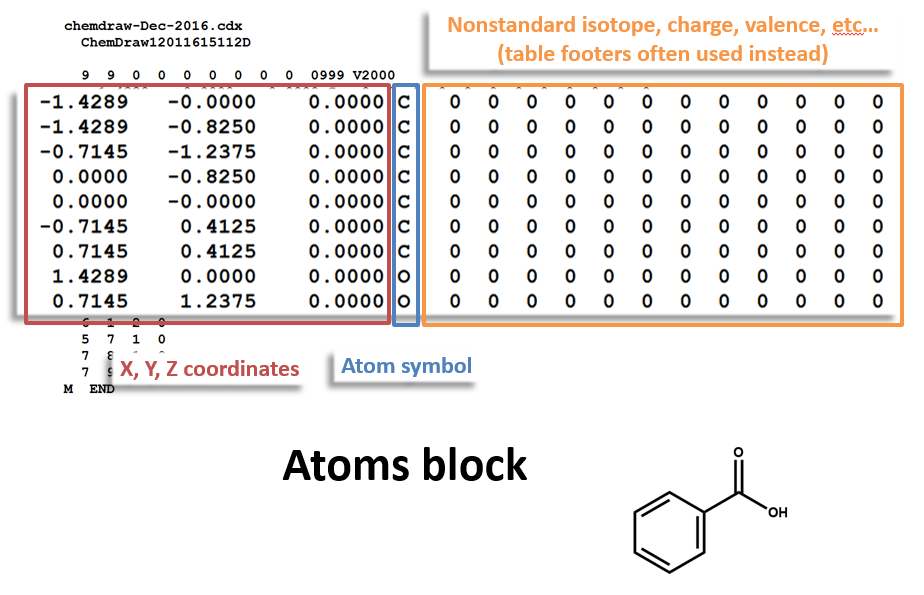
\includegraphics[scale=0.3]{imagenes/molfile.png}}  
    \caption{Contenido de un archivo MOL \cite{molfile_example}} 
\end{figure}


\subsection{Fuentes y bases de datos}

El gran número de facetas que presenta la información química necesita sistemas de almacenamiento a la altura. La química fue una de las primeras ramas científicas en utilizar bases de datos para almacenar: la cantidad de datos que se generaba creció rápidamente, y sigue creciendo hoy en día. 

Aunque es complicado clasificarlas, vamos a separarlas en tres grandes grupos según el tipo de información que almacenan: \cite{doi:10.1021/ci600234z}
\begin{itemize}
    \item \textbf{Bases de datos de publicaciones:} Pueden ser bibliográficas, guardando solamente los metadatos y la referencia a la publicación, o de texto completo, donde recogen la publicación de forma íntegra. %TODO: Qué son las publicaciones primarias?
    \item \textbf{Bases de datos fácticas:} Al contrario que las anteriores, que almacenan publicaciones de la literatura primaria, estas pueden guardar propiedades físicas de compuestos, información de espectroscopia, información legal, etc.
    \item \textbf{Bases de datos de estructuras y reacciones:} Recogen estructuras químicas, tanto individualmente como formando parte de reacciones. No se almacenan como imágenes, sino en formatos interpretables por la máquina.
    \item \textbf{Bases de datos de biología molecular:} Contienen secuencias de aminoácidos y nucleótidos.
\end{itemize}

Pero, ¿cómo podemos rellenarlas con datos? ¿De dónde podemos extraerlos ? Durante décadas se han publicado un gran número de artículos. Podríamos utilizarlos como una fuente muy amplia de información, ya que contienen todo el progreso científico. Específicamente para extraer datos relativos a estructuras, entran en juego utilidades conocidas como OCSR (Optical Chemical Structure Recognition).

Son capaces de transformar una imagen en un formato compatible con la máquina, como podría ser SMILES. En muchos casos incluso es posible introducirles una publicación completa y ellas mismas localizan las imágenes de moléculas. Con el paso del tiempo se han ido perfeccionando, y algunas son capaces de detectar información estereoquímica o de relacionar el compuesto con el texto de la publicación. Más adelante repasaremos algunas de estas utilidades. 

Por último, mencionar una base de datos que merece la pena conocer. Creada por el National Institute of Health (NIH), PubChem es una base de datos abierta que cada mes sirve a millones de usuarios en todo el mundo. Es una base de datos de estructuras y aunque contiene mayoritariamente moléculas pequeñas, también almacena nucleótidos, carbohidratos, lípidos, péptidos y macromoléculas modificadas químicamente. Para cada compuesto almacena su estructura, identificadores, propiedades físicas y químicas, toxicidad, patentes, etc. Los datos que aglutina provienen de diversas fuentes, como son agencias del gobierno estadounidense, editores de revistas científicas o proveedores químicos, aunque hay muchas más. \cite{pubchem}

\subsection{Métodos de búsqueda}
Almacenar información en las bases de datos no sirve de nada si no se desarrollan métodos eficientes para extraerla. En aquellas bases de datos donde se almacenan estructuras químicas, una de las principales formas de obtener información es buscar similitudes entre una molécula dada como entrada y otras que se encuentran almacenadas, de forma que compartan una subestructura específica o tengan otras características en común. Para ello, es clave la codificación de los compuestos.

También, si se almacenan metadatos y la base de datos está indexada sobre ellos se podría buscar por su nombre, etiquetas, etc. \cite{doi:10.1021/ci600234z}

\subsection{Métodos para análisis de datos}
En química, grandes cantidades de datos son producidas. Una vez que hemos conseguido limpiarlos y ordenarlos, tenemos un conocimiento muy valioso en nuestras manos. La información es muy interesante en sí misma, pero también lo son las relaciones que se esconden en su interior. Para ello, se crean modelos que puedan interiorizarlas.

El análisis de datos no solo se enfrenta a la extracción de la información principal, sino que también intenta generar nueva información secundaria. \cite{doi:10.1021/ci600234z}

Este TFG se desarrolla dentro de este ámbito, ya que, como describiremos más adelante, entrenamos un modelo capaz de detectar que imágenes contienen moléculas organometálicas. Además, creamos un modelo generativo para aumentar el tamaño del dataset en uso.

\newpage
\section{Deep learning}
En las últimas décadas, la Inteligencia Artificial (I.A) ha vivido un periodo de crecimiento brutal. Dentro del ámbito de la I.A. se engloban técnicas muy diferentes que tienen como objetivo simular el comportamiento inteligente de los seres vivos, siendo uno de sus rasgos la capacidad de aprendizaje. Los sistemas expertos fueron su primer éxito comercial. En ellos se codificaban una serie de reglas manualmente, emulando el razonamiento de un experto en un problema específico.

El aprendizaje automático es un subconjunto dentro de la Inteligencia Artificial. Aglutina aquellas técnicas que permiten a un ordenador construir modelos a partir de conjuntos de datos, aprendiendo con la experiencia. No hace falta definir reglas de forma explícita. Pero tiene un inconveniente, y es que en muchos casos un especialista humano tiene que elegir manualmente que características de los datos son relevantes en el problema.

El aprendizaje profundo o deep learning va un paso más allá. Es un subconjunto del aprendizaje automático, pero en las técnicas que engloba no es necesario indicar al modelo  las características útiles, ya que él mismo las descubre automáticamente. Y no se queda ahí, va un paso más allá, puede generar nuevas características a partir de las existentes.

El desarrollo temporal de estas técnicas coincide con el orden en el que las menciono. Como se puede apreciar, el proceso de aprendizaje consta de diferentes fases, de las que cada vez se encuentra automatizado un mayor número. \cite{berzal2018redes}

Casi todos los algoritmos de deep learning son una adaptación particular de un proceso que se puede resumir en los siguientes cuatro pasos:

\begin{itemize}
    \item Extraer un conjunto de datos asociado al problema (un conjunto de gran tamaño, cuanto más grande mejor).
    \item Diseñar una función de coste apropiada (loss function).
    \item Crear un modelo y definir sus hiperparámetros (tamaño, tasa de aprendizaje...), asignándole los valores más adecuados.
    \item Aplicar un algoritmo de optimización para minimizar la función de coste.
\end{itemize}

Siendo esta la estrategia que se utiliza en otras muchas técnicas de aprendizaje automático. La diferencia entre el deep learning y estas otras es la capacidad de abstracción que tiene el primero, que viene dada por la capacidad de jerarquizar la información en distintas capas utilizando múltiples niveles de representación. Esta abstracción permite separar la esencia de lo prescindible, de forma que los modelos pueden aprender qué relaciones entre los datos son importantes y cuáles son simples accidentes, y consecuentemente generalizar de forma adecuada. \cite{berzal2018redes}

\subsection{Redes neuronales multicapa}
Nuestro cerebro contiene un tipo especial de células llamadas neuronas. Estas reciben impulsos eléctricos que son capaces de atenuar o amplificar para posteriormente enviarlos a otras neuronas. La unión de millones de estas crea una estructura neuronal que es la que nos permite pensar y actuar como seres inteligentes.

En la informática se ha intentado emular este comportamiento, creando lo que se conoce como redes neuronales artificiales. Las neuronas artificiales omiten muchas características que definen a las biológicas, como su localización espacial, los retardos en la propagación de señales o los mecanismos químicos de sodio y potasio que permiten la transmisión de potenciales eléctricos. Al final, un modelo es una representación de la realidad, y por tanto contiene información más limitada que esta. El modelo de integración y disparo define la base de la neurona que se utiliza habitualmente en Inteligencia Artificial:

\begin{figure}[H]
\centering
    \fbox{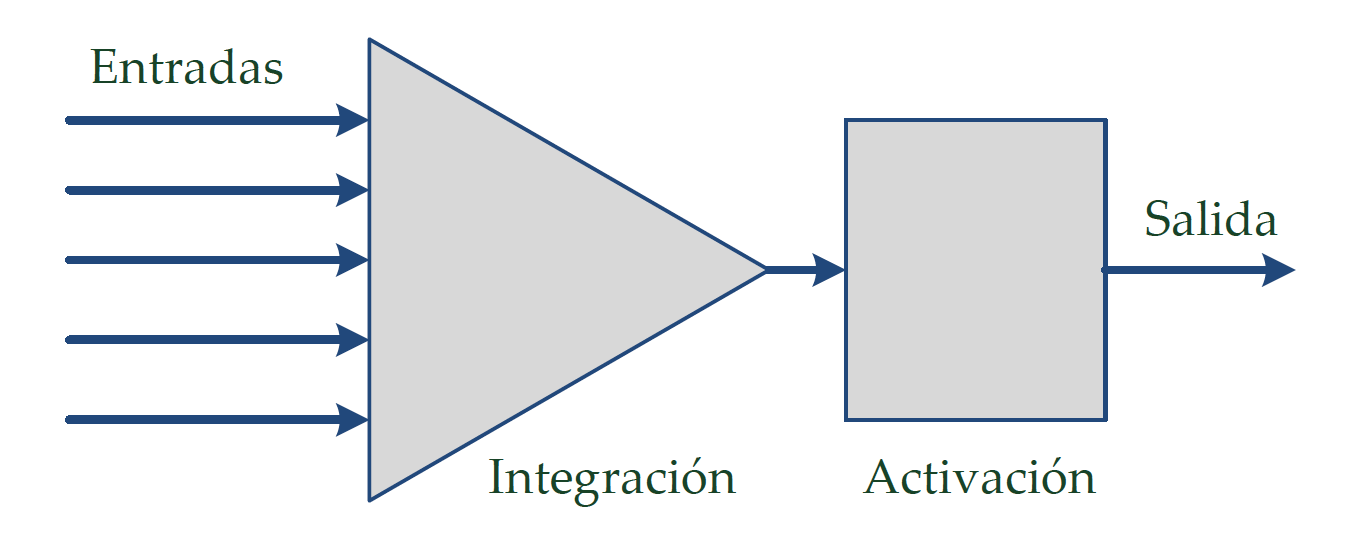
\includegraphics[scale=0.4]{imagenes/integracion_disparo.png}}  
    \caption{Modelo de integración y disparo en las neuronas artificiales \cite{berzal2018redes}} 
\end{figure}

En la fase de integración se unifican todas las señales $x_i$ entrantes a la neurona $j$, cada una influyendo en mayor o menor medida según el peso $w_{ij}$, peso de la conexión de la neurona $i$ hasta la neurona $j$:

\begin{equation}
    z_j = b_j + \sum_{i=1}^{n} x_iw_{ij}
\end{equation}

Además, en muchas ocasiones se añade la componente $b_j$ que actúa como sesgo, permitiendo que la salida de la neurona se desplace a la izquierda o a la derecha en el eje X. Este sesgo también se puede representar de forma implícita, de forma que $i$ parte de 0 en vez de 1, siendo $x_0 = 1$ y $w_0j = b_j$. \cite{berzal2018redes}

Pero esta fase de integración no es suficiente para simular el comportamiento del cerebro humano, su resultado es lineal. Una red neuronal se genera encadenando capas de estas neuronas, donde la salida de las neuronas de una capa actúan de entrada a las neuronas de la siguiente capa. La combinación de funciones lineales es una función lineal, y por tanto el resultado final de la red seguiría siendo una función lineal de las entradas. En definitiva, tener $n$ capas equivaldría a utilizar una única capa.

Es por ello que existe una segunda fase en este proceso, la fase de activación. Al resultado de integración en cada neurona se le aplica una función de activación no lineal ($\sigma$). A partir de ahora, nuestra red podrá aproximar funciones no lineales: cuantas más capas se utilicen en una red, con mayor precisión se podrá llevar a cabo esta aproximación.

\begin{equation}
    f_j = \sigma(z_j) = \sigma(b_j + \sum_{i=1}^{n} x_iw_{ij})
\end{equation}

\noindent $f_j$ es la salida final de la neurona. \cite{berzal2018redes}

\subsection{Redes neuronales convolutivas}
Si hay una técnica del aprendizaje profundo que funcione especialmente bien en la práctica, son las redes neuronales convolutivas o convolutional neural networks (CNN). Estas se utilizan para procesar señales, como son las imágenes.

Una ventaja frente a las redes multicapa reside en que pueden trabajar con entradas y salidas estructuradas. Esto supone que, en vez de recibir un vector de entradas correspondientes a diferentes variables, pueden trabajar directamente con un vector 1D, una matriz 2D o con un tensor con múltiples dimensiones. \cite{berzal2018redes} 

En estas redes, las capas realizan la operación de convolución en vez de la multiplicación de las entradas por pesos. En el caso de imágenes (señal 2D), esta operación se define como:

\begin{equation}
    S(i,j) = (I*K)(i,j) = \sum_m \sum_n I(m,n)K(i-m,j-n)
\end{equation}

Donde $I$ representa una imagen y $K$ un kernel de dos dimensiones \cite{Goodfellow-et-al-2016}. El tipo de convolución que describimos aquí es la discreta y por ello en la fórmula aparecen sumatorias, en vez de las integrales típicas de dominios continuos. En la siguiente figura se puede observar un ejemplo de convolución:

\begin{figure}[H]
\centering
    \fbox{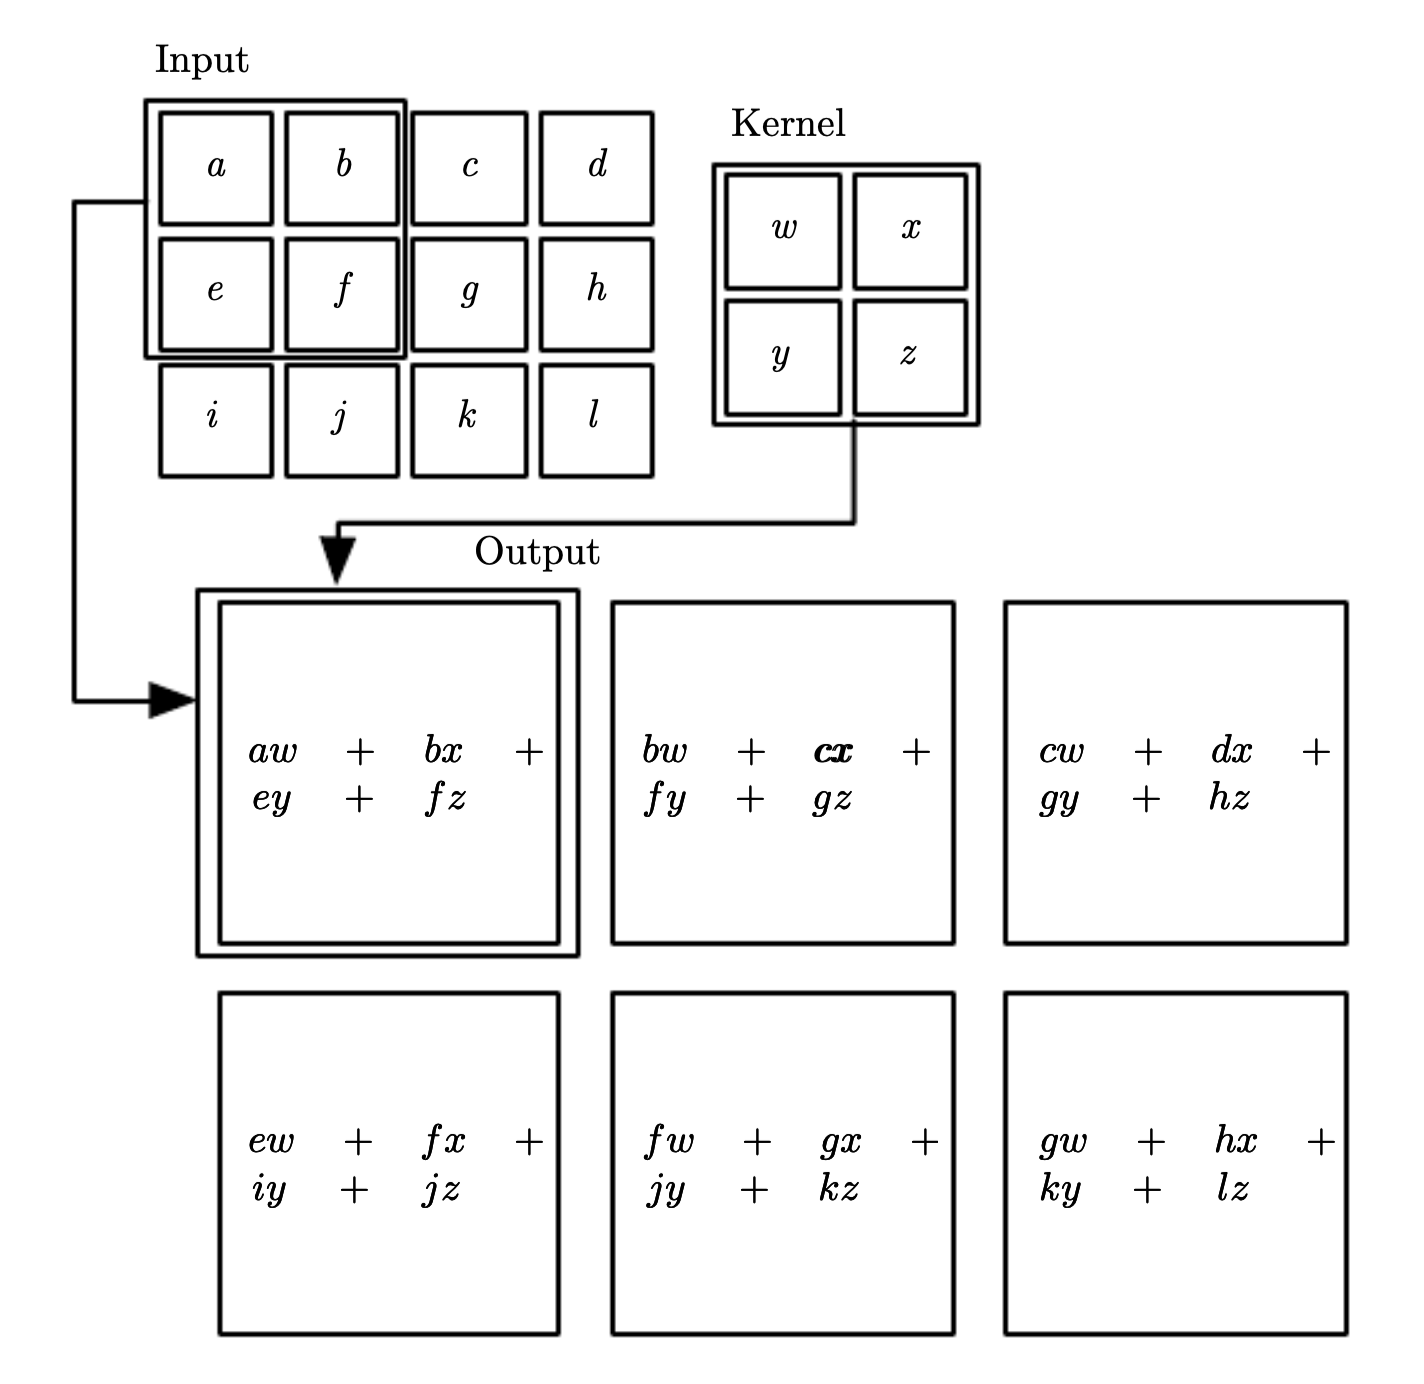
\includegraphics[scale=0.4]{imagenes/convolution.png}}  
    \caption{Resultado de convolucionar la entrada I con el kernel K \cite{Goodfellow-et-al-2016}}
\end{figure}

El kernel se va desplazando por la imagen, solapándose sobre cierta área de esta. En cada una de las posiciones que toma genera un valor de salida, fruto de la multiplicación del valor de los píxeles de la imagen sobre los que se encuentra por los pesos del kernel. Todos estos valores de salida forman el resultado final, que mantiene la misma estructura 2D (aunque normalmente con un menor tamaño). 

Así es como funcionan las redes neuronales convolutivas, donde cada capa de la red aplica este operador a la entrada que recibe. Con ellas:
\begin{itemize}
    \item Se reduce el número de parámetros necesarios. Este depende del tamaño de los kernel utilizados, que suele ser muy inferior al de las imágenes de entrada.
    \item Se mantienen las relaciones espaciales/temporales de las señales. Muy beneficioso en análisis de imágenes, donde dos pixeles cercanos contendrán información similar. Los capas convolutivas son capaces de interpretar estas relaciones y mantenerlas para las siguientes fases del modelo. \cite{Goodfellow-et-al-2016}
\end{itemize}

\subsection{Autocodificadores}
Los autocodificadores o autoencoders son un modelo de aprendizaje no supervisado que permite encontrar una representación latente no lineal para una distribución de datos dada.

Para comprenderlos correctamente, definamos primero lo que es una representación latente. Esta es una representación subyacente para una determinada distribución de datos, es decir, una forma ``comprimida" de representar la distribución que siguen estos datos. En esta representación, se reduce el número de dimensiones necesarias para definir la distribución.

Existe un algoritmo conocido como análisis de componentes principales (Principal Component Analysis, PCA) que encuentra una transformación lineal de la representación original a otra latente. Pero tiene un problema, y es que como su definición indica esta transformación es lineal. \cite{vqvae}

Los autocodificadores realizan esta tarea pero encontrando una transformación no lineal, por lo que pueden trabajar con datos más complejos. Para ello constan de dos partes, el codificador y el decodificador:

\begin{figure}[H]
\centering
    \fbox{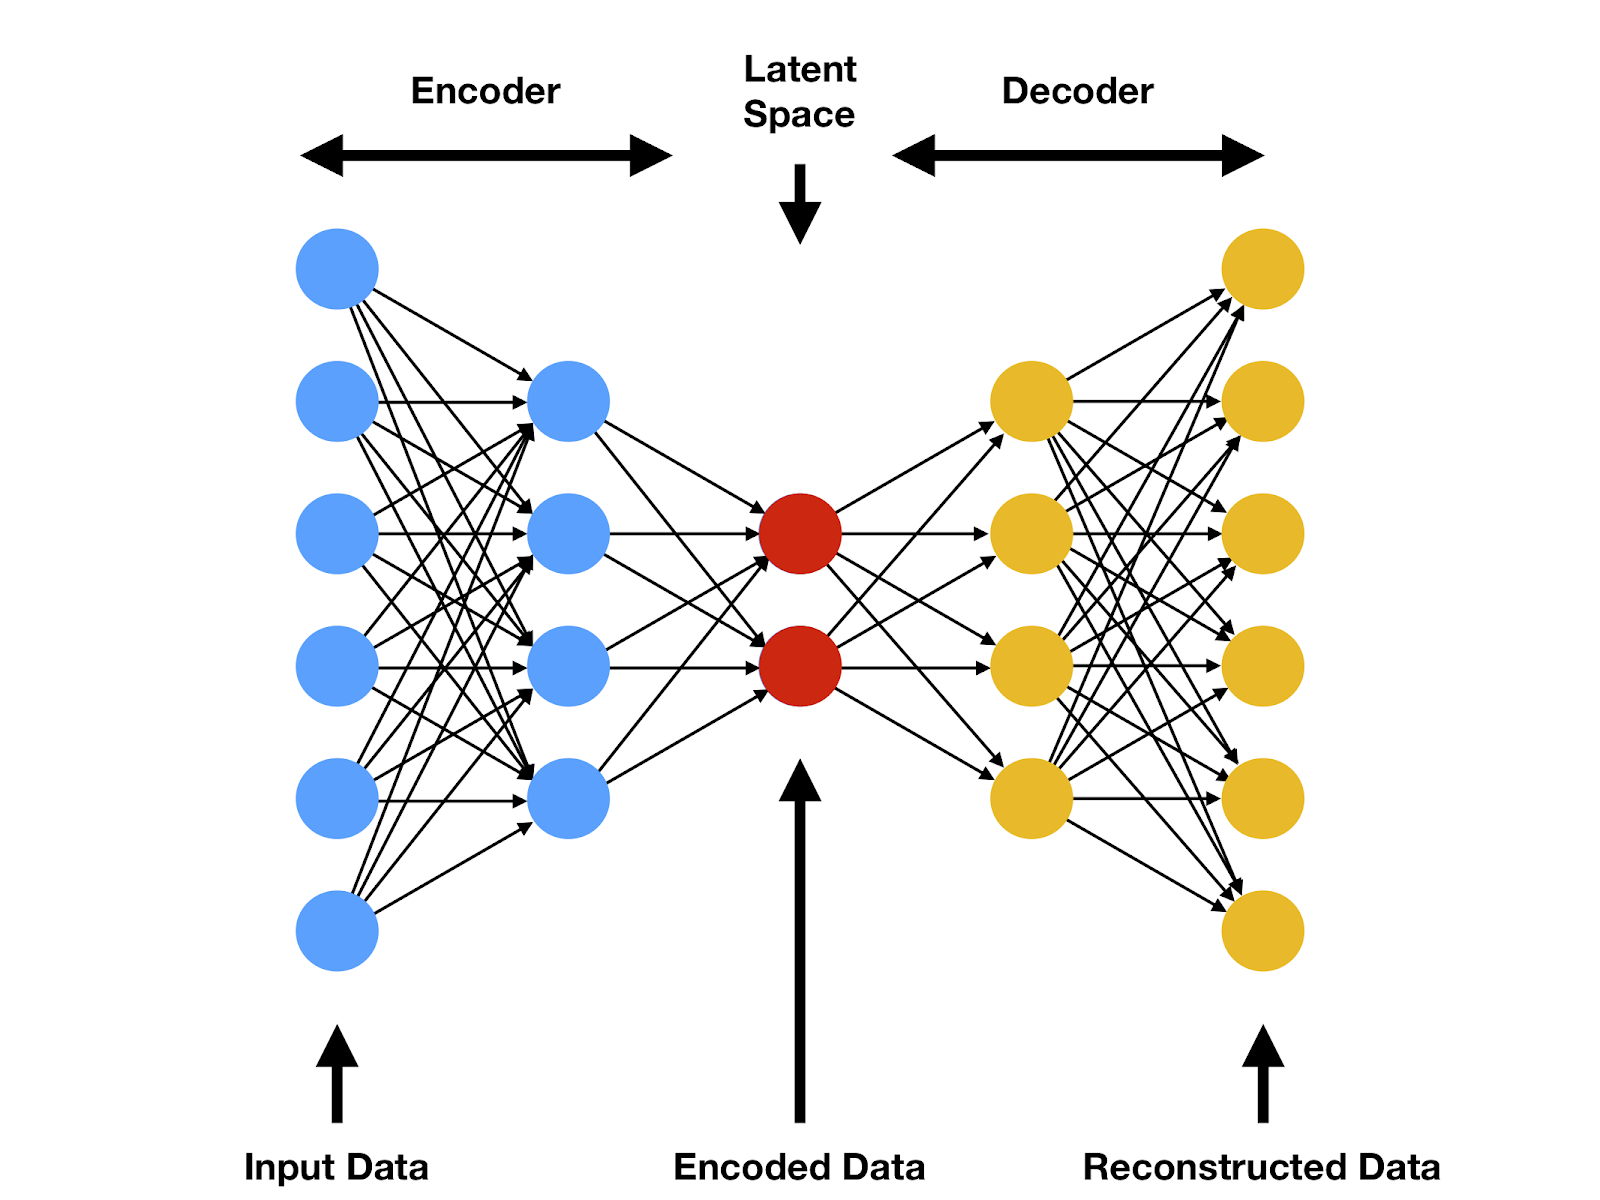
\includegraphics[scale=0.18]{imagenes/autoencoder.png}}  
    \caption{Secciones en las que se divide un autocodificador \cite{vqvae}}
\end{figure}

El objetivo tras el entrenamiento del modelo es que los datos reconstruidos por el decodificador sean lo más parecidos posible a los de entrada.

Un tipo especial de autocodificador es el autocodificador variacional (Variational Autoencoder, VAE). La principal diferencia viene dada por la estructura que sigue la representación latente, donde se fuerza al autocodificador a organizarla de forma que puntos de datos similares se encuentren cerca en la representación latente y puntos diferentes se encuentren separados. En un autocodificador regular esto no se exige, por lo que no podríamos desplazarnos por el espacio latente y observar cambios graduales que se corresponden con cambios graduales en la representación original. \cite{vqvae}

\begin{figure}[H]
\centering
    \fbox{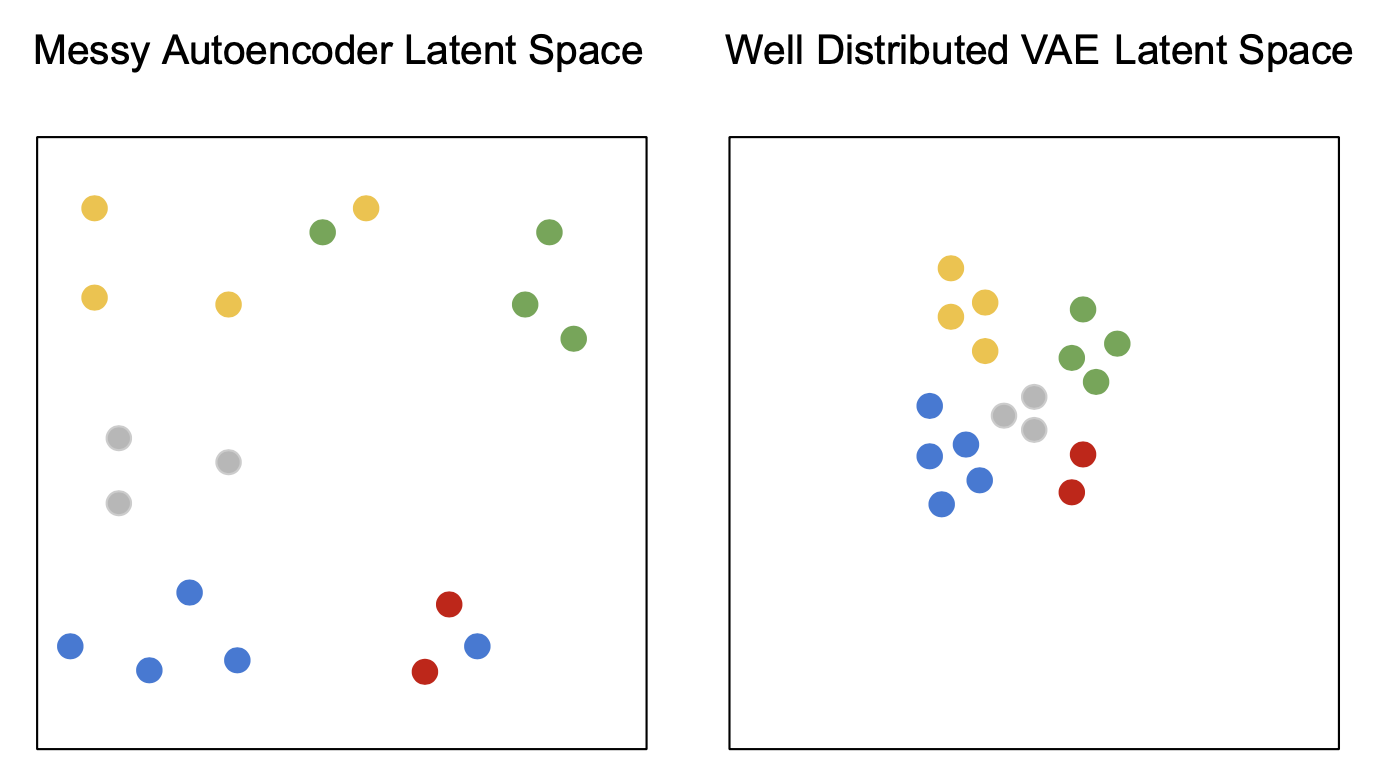
\includegraphics[scale=0.23]{imagenes/vae.png}}  
    \caption{Espacio latente en un autocodificador regular vs en VAE \cite{vqvae}}
\end{figure}

\subsubsection{Vector Quantized Variational Autoencoder}
La representación latente por defecto en los VAE es continua. Pero existe una variante en la que se discretiza esta representación. Esto es útil cuando trabajamos con datos como imágenes: podría utilizarse una variable discreta para el color, otra para el tipo de objeto, su tamaño, etc. Muchos otros elementos del mundo real son susceptibles de representarse de forma discreta. Hay modelos como los transformers, que vamos a estudiar más adelante, que están diseñados para trabajar sobre datos con esta codificación.

Los Vector Quantized Variational Autoencoders (VQVAE) utilizan este tipo de codificación, donde la representación latente consiste en lo que se conoce como libro de código (codebook). Este codebook no deja de ser un conjunto de vectores discretos asociados a un índice.

Cuando el codificador recibe un dato, este se transforma a la representación latente. A continuación, se introduce al decodificador el vector del codebook con el que existe una menor distancia euclídea. Este vector es procesado por el decodificador devolviendo la salida final. Dicho esto, se podría pensar que la potencia expresiva del autoencoder es muy baja, ya que el número de vectores del codebook es mucho más pequeño que el conjunto de posibles datos de entrada, y siempre que se introdujese el mismo vector al decodificador obtendríamos la misma salida.

Esto no es así, ya que normalmente no se utiliza un único vector: en datos como imágenes, es probable que se escoja un conjunto de vectores que se introducen en el decodificador. Estos son procesados conjuntamente y finalmente se devuelve la imagen sintética. De esta forma, el número de posibilidades crece enormemente. \cite{vqvae}

\subsection{Redes generativas antagónicas}
En inglés conocidas como Generative Adversarial Networks (GANs), son un tipo de modelos utilizados para generar datos sintéticos, que por ejemplo pueden servir para ampliar nuestro dataset. Contienen dos módulos que trabajan simultáneamente, cada uno de ellos intentando ser mejor que el otro. Estos dos módulos son el generador G y el discriminador D: el generador intenta crear datos sintéticos parecidos a los reales y el discriminador actuará de juez, tendrá que decidir si dado un dato este es real o sintético.
Estamos en un juego en el que el generador intentará mejorar todo lo posible para generar imágenes indistinguibles a ojos del discriminador, desarrollándose en dos escenarios:

\begin{itemize}
    \item Se muestrean datos x del conjunto de entrenamiento y se introducen en D. En este caso, D(x) será un valor cercano a 1, ya que las muestras son datos reales.
    \item Se introduce en G una muestra z generada aleatoriamente de acuerdo a una distribución de probabilidad, siendo G(z) una muestra sintética. D(G(z)) deberá tomar un valor cercano a 0, detectando que no se trata de una muestra real. Sin embargo, aunque el discriminador actúa para que D(G(z)) sea cercano a 0, el generador hace todo lo contrario y pretende que D(G(z)) se aproxime a 1.
\end{itemize}

El entrenamiento se lleva a cabo simultáneamente en G y D, actualizando los pesos de ambos en cada iteración. Este termina cuando se ha alcanzado un equilibrio en el que ni al generador ni al discriminador les interesa modificar sus pesos, llamado equilibrio de Nash.

Las GANs son muy populares actualmente y se pueden utilizar con diferentes tipos de datos, entre ellos las imágenes. Originalmente las GANs se presentaron utilizando capas completamente conectadas (fully connected layers), pero la técnica de las redes neuronales convolutivas también se aplicó a las GANs dando lugar a las Deep Convolutional GAN (DCGAN). \cite{berzal2018redes}

\subsection{Transformers}
En los últimos años, se han desarrollado diferentes estrategias que permiten el modelado de secuencias. Algunas de ellas son las Redes Neuronales Recurrentes (RNN), los LSTM o modelos basados en redes convolutivas, como Wavenet. Aunque han dado buenos resultados en campos como la generación de texto, son mejorables, ya que las técnicas de memoria que implementan solo les permiten recordar los últimos datos de la secuencia. Así, en sucesiones de mayor longitud, no podrán mantener en memoria datos alejados del punto actual.

Para resolver este problema, los investigadores han creado lo que se conoce como mecanismos de atención. En ellos, el modelo es capaz de comprender qué datos de la secuencia son importantes para la tarea que estamos desarrollando. Estos datos son los que memoriza, descartando el resto. Funcionan de forma similar a nuestro cerebro: cuando vemos una imagen, aunque parece que estamos contemplando todos sus detalles, solo estamos prestando atención a fragmentos concretos de esta y obviando los detalles en el resto de áreas. Algunos autores aplicaron esta técnica a arquitecturas ya existentes. 

Pero en 2017, Vaswani et al. \cite{vaswani2017attention} propone un modelo basado únicamente en mecanismos de atención, prescindiendo de técnicas como la recurrencia o las convoluciones: a esta arquitectura la llamó el Transformer. El modelo está formado por 6 codificadores y 6 decodificadores:

\begin{figure}[H]
\centering
    \fbox{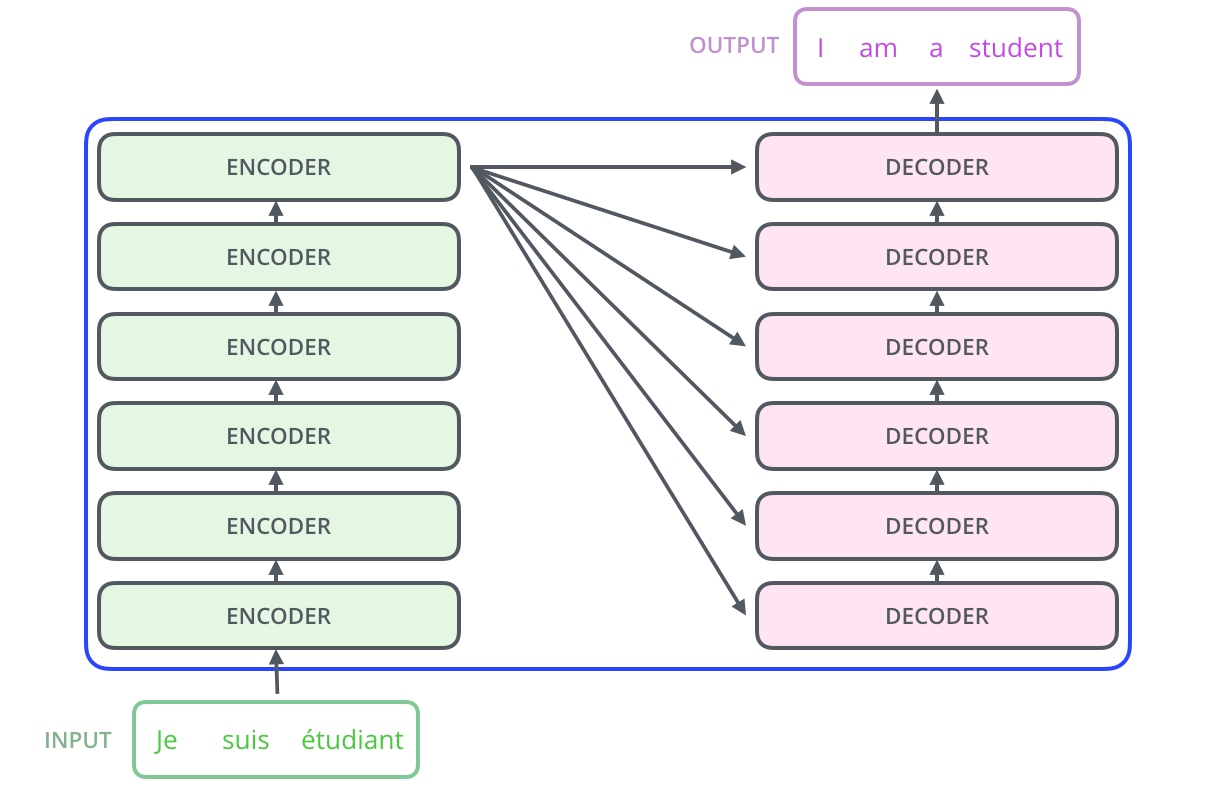
\includegraphics[scale=0.25]{imagenes/transformer.png}}  
    \caption{Transformer aplicado a la generación de texto \cite{transformers}}
\end{figure}

En cada codificador, las características de entrada primero pasan por una capa de auto-atención, en la que interactúan entre sí y se descubre a cuáles hay que prestar mayor atención. La salida de esta primera capa serán los datos agregados resultantes de esas interacciones y las puntuaciones de atención. A continuación, se introduce esta salida en una red neuronal completamente conectada. \cite{self-attention}

Los decodificadores también poseen estas dos capas, pero entre ambas existe otra capa de atención que ayuda al decodificador a concentrarse en las características importantes de la entrada.

\begin{figure}[H]
\centering
    \begin{subfigure}{.85\textwidth}
        \centering
        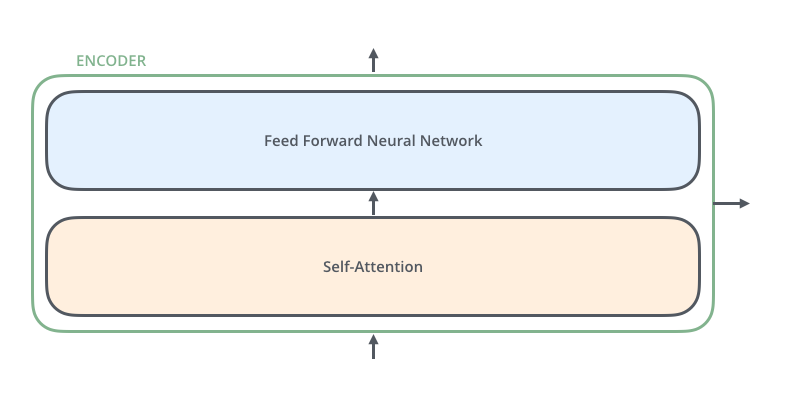
\includegraphics[width=1\linewidth]{imagenes/transformer_encoder.png}
        \caption{Estructura interior del codificador}
        \label{fig:sub1}
    \end{subfigure}%

    \bigskip

    \begin{subfigure}{.5\textwidth}
        \centering
        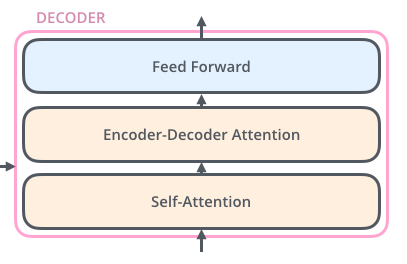
\includegraphics[width=1\linewidth]{imagenes/transformer_decoder.png}
        \caption{Estructura exterior del decodificador}
    \end{subfigure}

    \caption{Los dos tipos de capas que forman el Transformer \cite{transformers}}
\end{figure}


Los Transformer son actualmente los modelos más efectivos en tareas como la generación de lenguaje natural, y también se han aplicado a generación de imágenes. Estos son capaces de memorizar datos de cualquier punto de la secuencia, al contrario que otros modelos recurrentes o convolutivos, que sólo almacenan las interacciones locales. \cite{transformers}



\newpage
\section{Bibliotecas y paquetes}
En el estado del arte encontramos productos desarrollados por investigadores que nos van a facilitar cumplir nuestro objetivo. 

\subsection{Taming Transformers for High-Resolution Image Synthesis}
Científicos de la Universidad de Heidelberg (Alemania) publicaron a finales de 2020 un modelo capaz de generar imágenes sintéticas de alta resolución utilizando transformers. En publicaciones previas ya se habían expuesto modelos generativos basados en transformers \cite{chen2020generative}, pero estos solo podían funcionar con imágenes de pequeño tamaño. El coste computacional de un transformer aplicado directamente en imágenes crece cuadráticamente con el tamaño de esta, así que no es viable utilizarlos en imágenes de más de 100x100 píxeles, y mucho menos en aquellas del orden del megapixel.

P. Esser et al. \cite{esser2021taming} desarrolla un método capaz de combinar la potencia generativa de los transformers con la eficiencia que aportan las redes convolutivas. 

\begin{figure}[H]
\centering
    \fbox{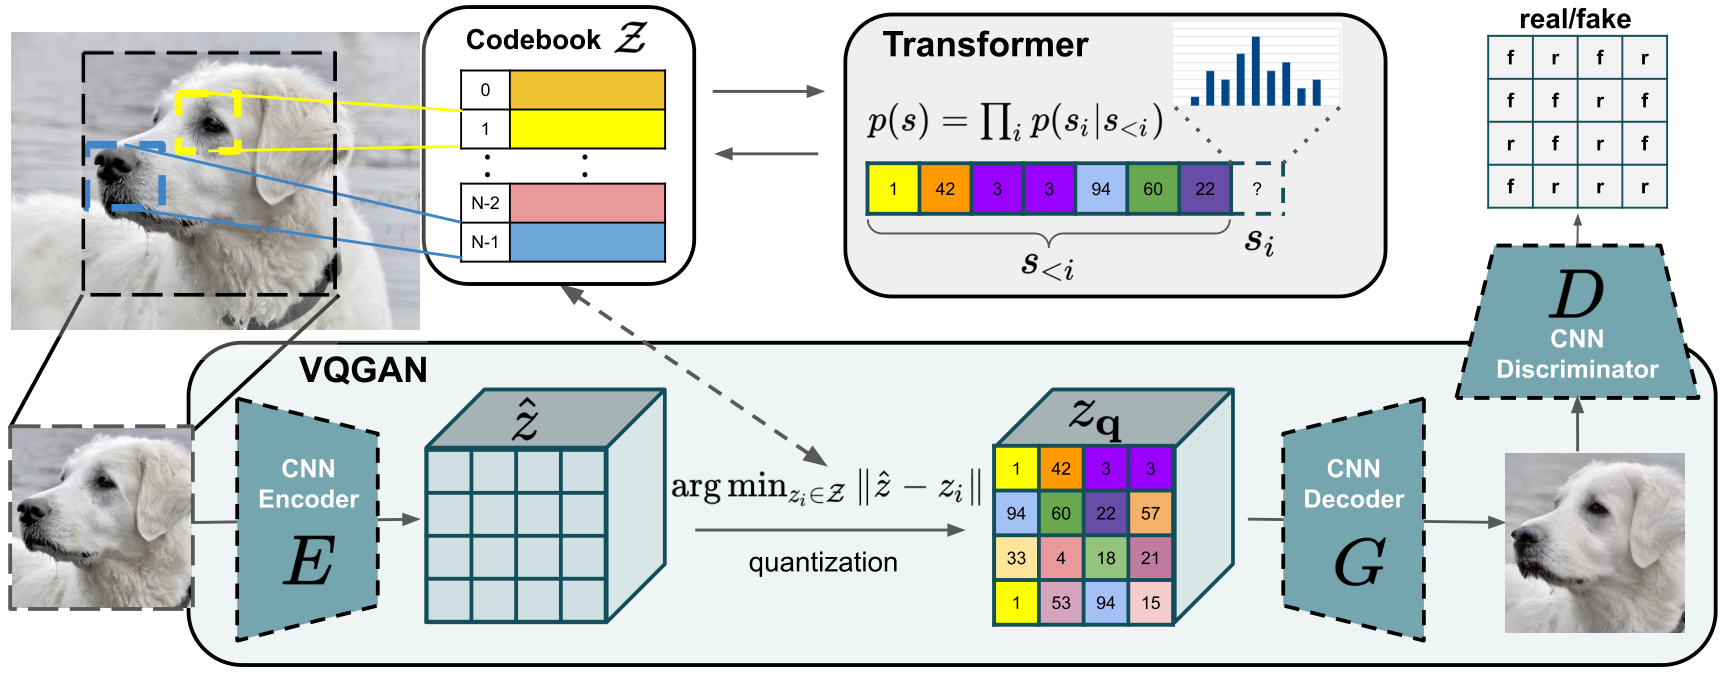
\includegraphics[scale=0.5]{imagenes/taming.png}}  
    \caption{Modelo propuesto por P. Esser et al. \cite{esser2021taming}}
\end{figure}

La arquitectura convolutiva de la que hablamos es un Vector Quantized Generative Adversarial Network (VQGAN), una variante de VQVAE propuesta por los autores de la publicación donde la estructura codificador-decodificador del VAE se entrena mediante un procedimiento adversarial, utilizando un discriminador.

Tras entrenar el modelo, se habrá generado un codebook que comprime la información de las imágenes. Será sobre este codebook sobre el que se entrene el transformer que posteriormente nos permitirá sintetizar imágenes sintéticas. Ahora tendremos un modelo que es capaz de aprovechar la gran capacidad generativa de los transformers, manteniendo tiempos de entrenamiento razonables gracias a VQGAN.

En la publicación original los autores muestran ejemplos de los resultados que se pueden obtener dada una imagen condicional de entrada:

\begin{figure}[H]
\centering
    \fbox{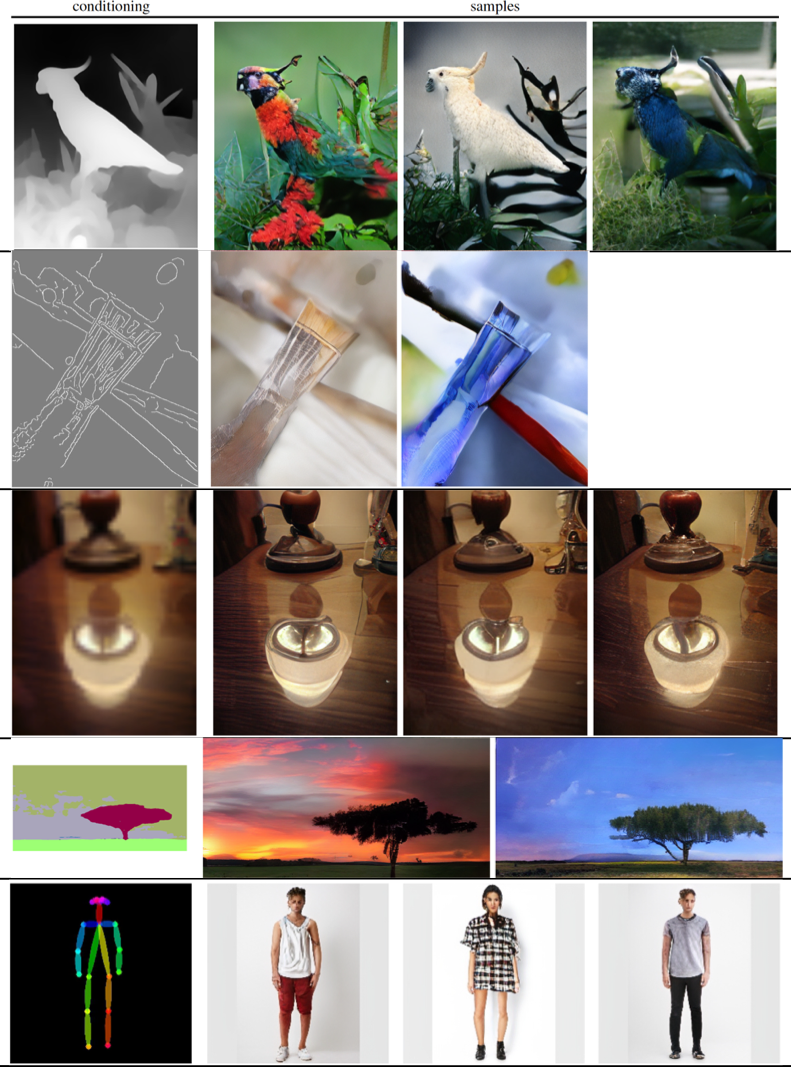
\includegraphics[scale=0.9]{imagenes/taming_examples.png}}  
    \caption{Ejemplos generados utilizando el modelo basado en transformer \cite{esser2021taming}}
\end{figure}

Se observa que funciona correctamente en diversas situaciones, por lo que puede ser una buena opción para nuestra tarea de síntesis de imágenes.

\subsection{Pytorch}
PyTorch es una biblioteca basada en tensores optimizada para crear modelos de aprendizaje profundo que se entrenen y ejecuten tanto en GPUs como en CPUs.

\begin{figure}[H]
\centering
    \fbox{
\includegraphics[scale=0.2]{imagenes/pytorch.jpeg}}  
    \caption{Logo de PyTorch}
\end{figure}

Es adecuada para ser utilizada en proyectos de investigación, ya que convierte el desarrollar y experimentar con nuevas arquitecturas en algo relativamente sencillo. Su núcleo proporciona la capacidad de definir funciones matemáticas y calcular sus gradientes.

Al compararla con otras bibliotecas de aprendizaje profundo como Tensorflow encontramos diferencias. Esta sigue el paradigma definición-compilación-ejecución, mientras que PyTorch presenta una estructura definición-ejecución, donde no existe una etapa de compilación. El usuario puede definir una expresión matemática y calcular su gradiente directamente. \cite{ketkar2017introduction}

A continuación, vamos a comentar algunas características y módulos incluidos en esta biblioteca que merece la pena conocer.

\subsubsection{Dataset y DataLoader}
El código para gestionar los datos con los que vamos a trabajar se puede volver complejo y difícil de mantener. PyTorch proporciona los módulos $torch.utils.data.DataLoader$ y $torch.utils.data.Dataset$ para automatizar la carga y la manipulación de los datos, tanto procedentes de datasets ya existentes (por ejemplo, MNIST) como de datos propios.

$torch.utils.data.Dataset$ es una clase heredada por una clase hija en la que se implementan ciertos métodos encargados de cargar los datos. Un dataset puede ser de tipo $iterable$ o de tipo $map$: los primeros implementan $\_\_iter\_\_()$, y permiten que el objeto sea iterable, de forma que $iter(dataset)$ devuelve un flujo de datos que están siendo leídos de una base de datos o incluso se están produciendo en tiempo real. Por otra parte, un dataset de tipo $map$ implementa los métodos $\_\_getitem\_\_()$ y $\_\_len\_\_()$. Esto permite establecer una relación clave-dato, donde si $CompoundDataset$ es un dataset con imágenes que pueden ser o no compuestos químicos, $CompoundDataset[idx]$ devolvería la imagen número $idx$ junto a su etiqueta. Este último tipo de dataset es el que utilizamos nosotros.

El constructor de un objeto de tipo $torch.utils.data.DataLoader$ recibe como principal argumento un objeto $torch.utils.data.Dataset$. También recibe otros parámetros, como el tamaño del batch o si queremos que los datos sean devueltos en un orden aleatorio. Devuelve un iterable que cumple estas características, lo que facilita en gran medida el entrenamiento de modelos. 

Utilizando estos módulos separamos los datos del código de entrenamiento, obteniendo una mayor modularidad y un código más fácil de leer. \cite{pytorch-doc}

\subsubsection{Módulos $torch.nn$ y $torch.optim$}
El primero contiene los principales componentes utilizados en la construcción de redes neuronales y otras arquitecturas de aprendizaje profundo. Algunos de estos son:

\begin{itemize}
    \item \textbf{torch.nn.Module:} Es la clase padre de la que heredan todas las implementaciones de redes neuronales. En su constructor, entre otros elementos, se pueden inicializar diferentes capas que serán utilizadas en el método $forward()$, donde se especifica la estructura de la red y las conexiones entre ellas.
    \item \textbf{torch.nn.functional:} Recoge funciones de activación, de error así como capas de la red que no tienen un estado asociado.
    \item \textbf{torch.nn.Conv2d}, \textbf{torch.nn.MaxPool2d}, \textbf{torch.nn.Linear} son ejemplos de capas contenidas en este módulo. Existen diferentes tipos de capas lineales, convolutivas, recurrentes, transformer, etc. previamente implementadas y listas para ser utilizadas.
\end{itemize}

Por otro lado, $torch.optim$ contiene optimizadores como son SGD o Adam, encargados de actualizar los parámetros del modelo durante el entrenamiento. \cite{pytorch-doc}

\subsubsection{Autograd}
Al entrenar redes neuronales, el método más utilizado para actualizar los parámetros del modelo es la propagación hacia atrás o back propagation. Estos se ajustan de acuerdo al gradiente de la función de error con respecto al parámetro dado.

PyTorch facilita la aplicación de la propagación hacia atrás a través del módulo $torch.autograd$. Cuando implementamos un modelo, solo es necesario declarar el método $forward()$, ya que PyTorch crea sobre la marcha el grafo de las operaciones necesarias para calcular el gradiente. Durante el entrenamiento del modelo, al llamar a $loss.backward()$ se calculará el gradiente utilizando este grafo. \cite{pytorch-doc}

Como conclusión, PyTorch aporta una gran flexibilidad para crear modelos de aprendizaje profundo, su sintaxis y paradigma de programación son relativamente fáciles de aprender y contiene un gran número de módulos que permiten crear modelos complejos. Aparte, es compatible con el entrenamiento en GPU y permite guardar los modelos entrenados. Por todas estas razones puede resultar una librería adecuada para implementar el clasificador de imágenes.